\chapter{Существующие решения}
\section{Критерии сравнения систем управления реестром}

На основе анализа современных тенденций контейнеризации и изучения возможностей системы Harbor как эталонного решения можно сформулировать комплекс требований к корпоративной системе управления реестром Docker-образов. Эти требования охватывают различные аспекты функционирования системы и будут использованы в качестве основы для сравнительного анализа существующих решений.

В области безопасности система должна обеспечивать многоуровневую защиту артефактов и инфраструктуры. Обязательным является наличие интегрированных механизмов сканирования уязвимостей с регулярным обновлением баз данных CVE и возможностью интеграции с различными сканерами. Система должна поддерживать цифровую подпись образов для гарантии их целостности и аутентичности, предотвращая использование скомпрометированных артефактов в production-среде. Гибкая система управления доступом на основе ролей (RBAC) с поддержкой интеграции с корпоративными системами аутентификации (LDAP, Active Directory, OIDC) позволяет централизованно управлять правами доступа в соответствии с организационной структурой \cite{harbor-docs}.

С точки зрения управления жизненным циклом артефактов, корпоративная система должна предоставлять инструменты для эффективного версионирования и тегирования образов, включая поддержку семантического версионирования и тегов \cite{docker-spec}. Автоматическое управление политиками хранения с возможностью настройки правил удаления устаревших образов на основе различных критериев (время, количество версий, теги) необходимо для оптимизации использования дискового пространства. Поддержка квот и ограничений на уровне проектов и пользователей предотвращает неконтролируемый рост объема данных и обеспечивает равномерное распределение ресурсов.

Для обеспечения высокой доступности и отказоустойчивости система должна предоставлять механизмы репликации между географически распределенными инстансами, поддерживая как синхронные, так и асинхронные режимы синхронизации. Возможности горизонтального масштабирования и балансировки нагрузки позволяют системе адаптироваться к росту числа пользователей и объема данных без потери производительности \cite{gartner2023}. Регулярное резервное копирование метаданных и образов с возможностью быстрого восстановления после сбоев является критически важным требованием для обеспечения непрерывности бизнес-процессов.

Интеграционные возможности системы должны обеспечивать взаимодействие с существующей инфраструктурой организации. Поддержка REST API для автоматизации процессов CI/CD позволяет интегрировать реестр в процессы непрерывной интеграции и доставки, ускоряя разработку и повышая ее надежность. Современный веб-интерфейс с интуитивной навигацией и комплексными возможностями управления упрощает ежедневную работу администраторов и разработчиков, снижая порог вхождения и уменьшая вероятность ошибок. Наличие инструментов командной строки и программных интерфейсов обеспечивает возможности для автоматизации задач управления и интеграции со скриптами и системами оркестрации.

Сформулированные требования представляют собой комплексный набор критериев, который будет использован для проведения сравнительного анализа систем управления реестрами контейнерных образов. Соответствие этим требованиям позволит объективно оценить пригодность различных решений для использования в корпоративной среде:

\begin{enumerate}
	\item cканирование уязвимостей - возможность автоматического обнаружения уязвимостей в контейнерных образах;
	\item цифровая подпись образов - поддержка механизмов гарантии целостности и аутентичности артефактов;
	\item RBAC - управление доступом на основе ролей с интеграцией корпоративных систем аутентификации;
	\item репликация - возможности синхронизации данных между геораспределенными инстансами;
	\item политики хранения - автоматическое управление жизненным циклом артефактов;
	\item квоты - установка ограничений на использование ресурсов;
	\item поддержка различных артефактов - работа не только с Docker-образами, но и с Helm-чартами, OCI-артефактами;
	\item интеграция с CI/CD - возможности взаимодействия с системами непрерывной интеграции и доставки;
	\item веб-интерфейс (UI) - наличие пользовательского интерфейса для управления реестром;
	\item API и CLI - программные интерфейсы для автоматизации задач управления.
\end{enumerate}

\section{Результаты сравнения}

Результаты комплексного сравнения 30 систем управления реестрами Docker-образов представлены в таблицах приложения А. Таблица демонстрирует уровень поддержки ключевых функций в различных категориях решений.

Для каждого параметра использовалась трехбалльная система оценки:
\begin{itemize}
	\item 2 - функция полностью поддерживается;
	\item 1 - функция поддерживается частично или требует дополнительной настройки;
	\item 0 - функция отсутствует.
\end{itemize}

\section{Анализ полученных результатов}

Для наглядного представления уровня поддержки ключевых функций среди рассмотренных систем были построена аналитическая диаграмма. 

На рисунке~\ref{fig:support-analysis} представлена диаграмма сравнения поддержки ключевых функций.

\begin{figure}[H]
	\centering
	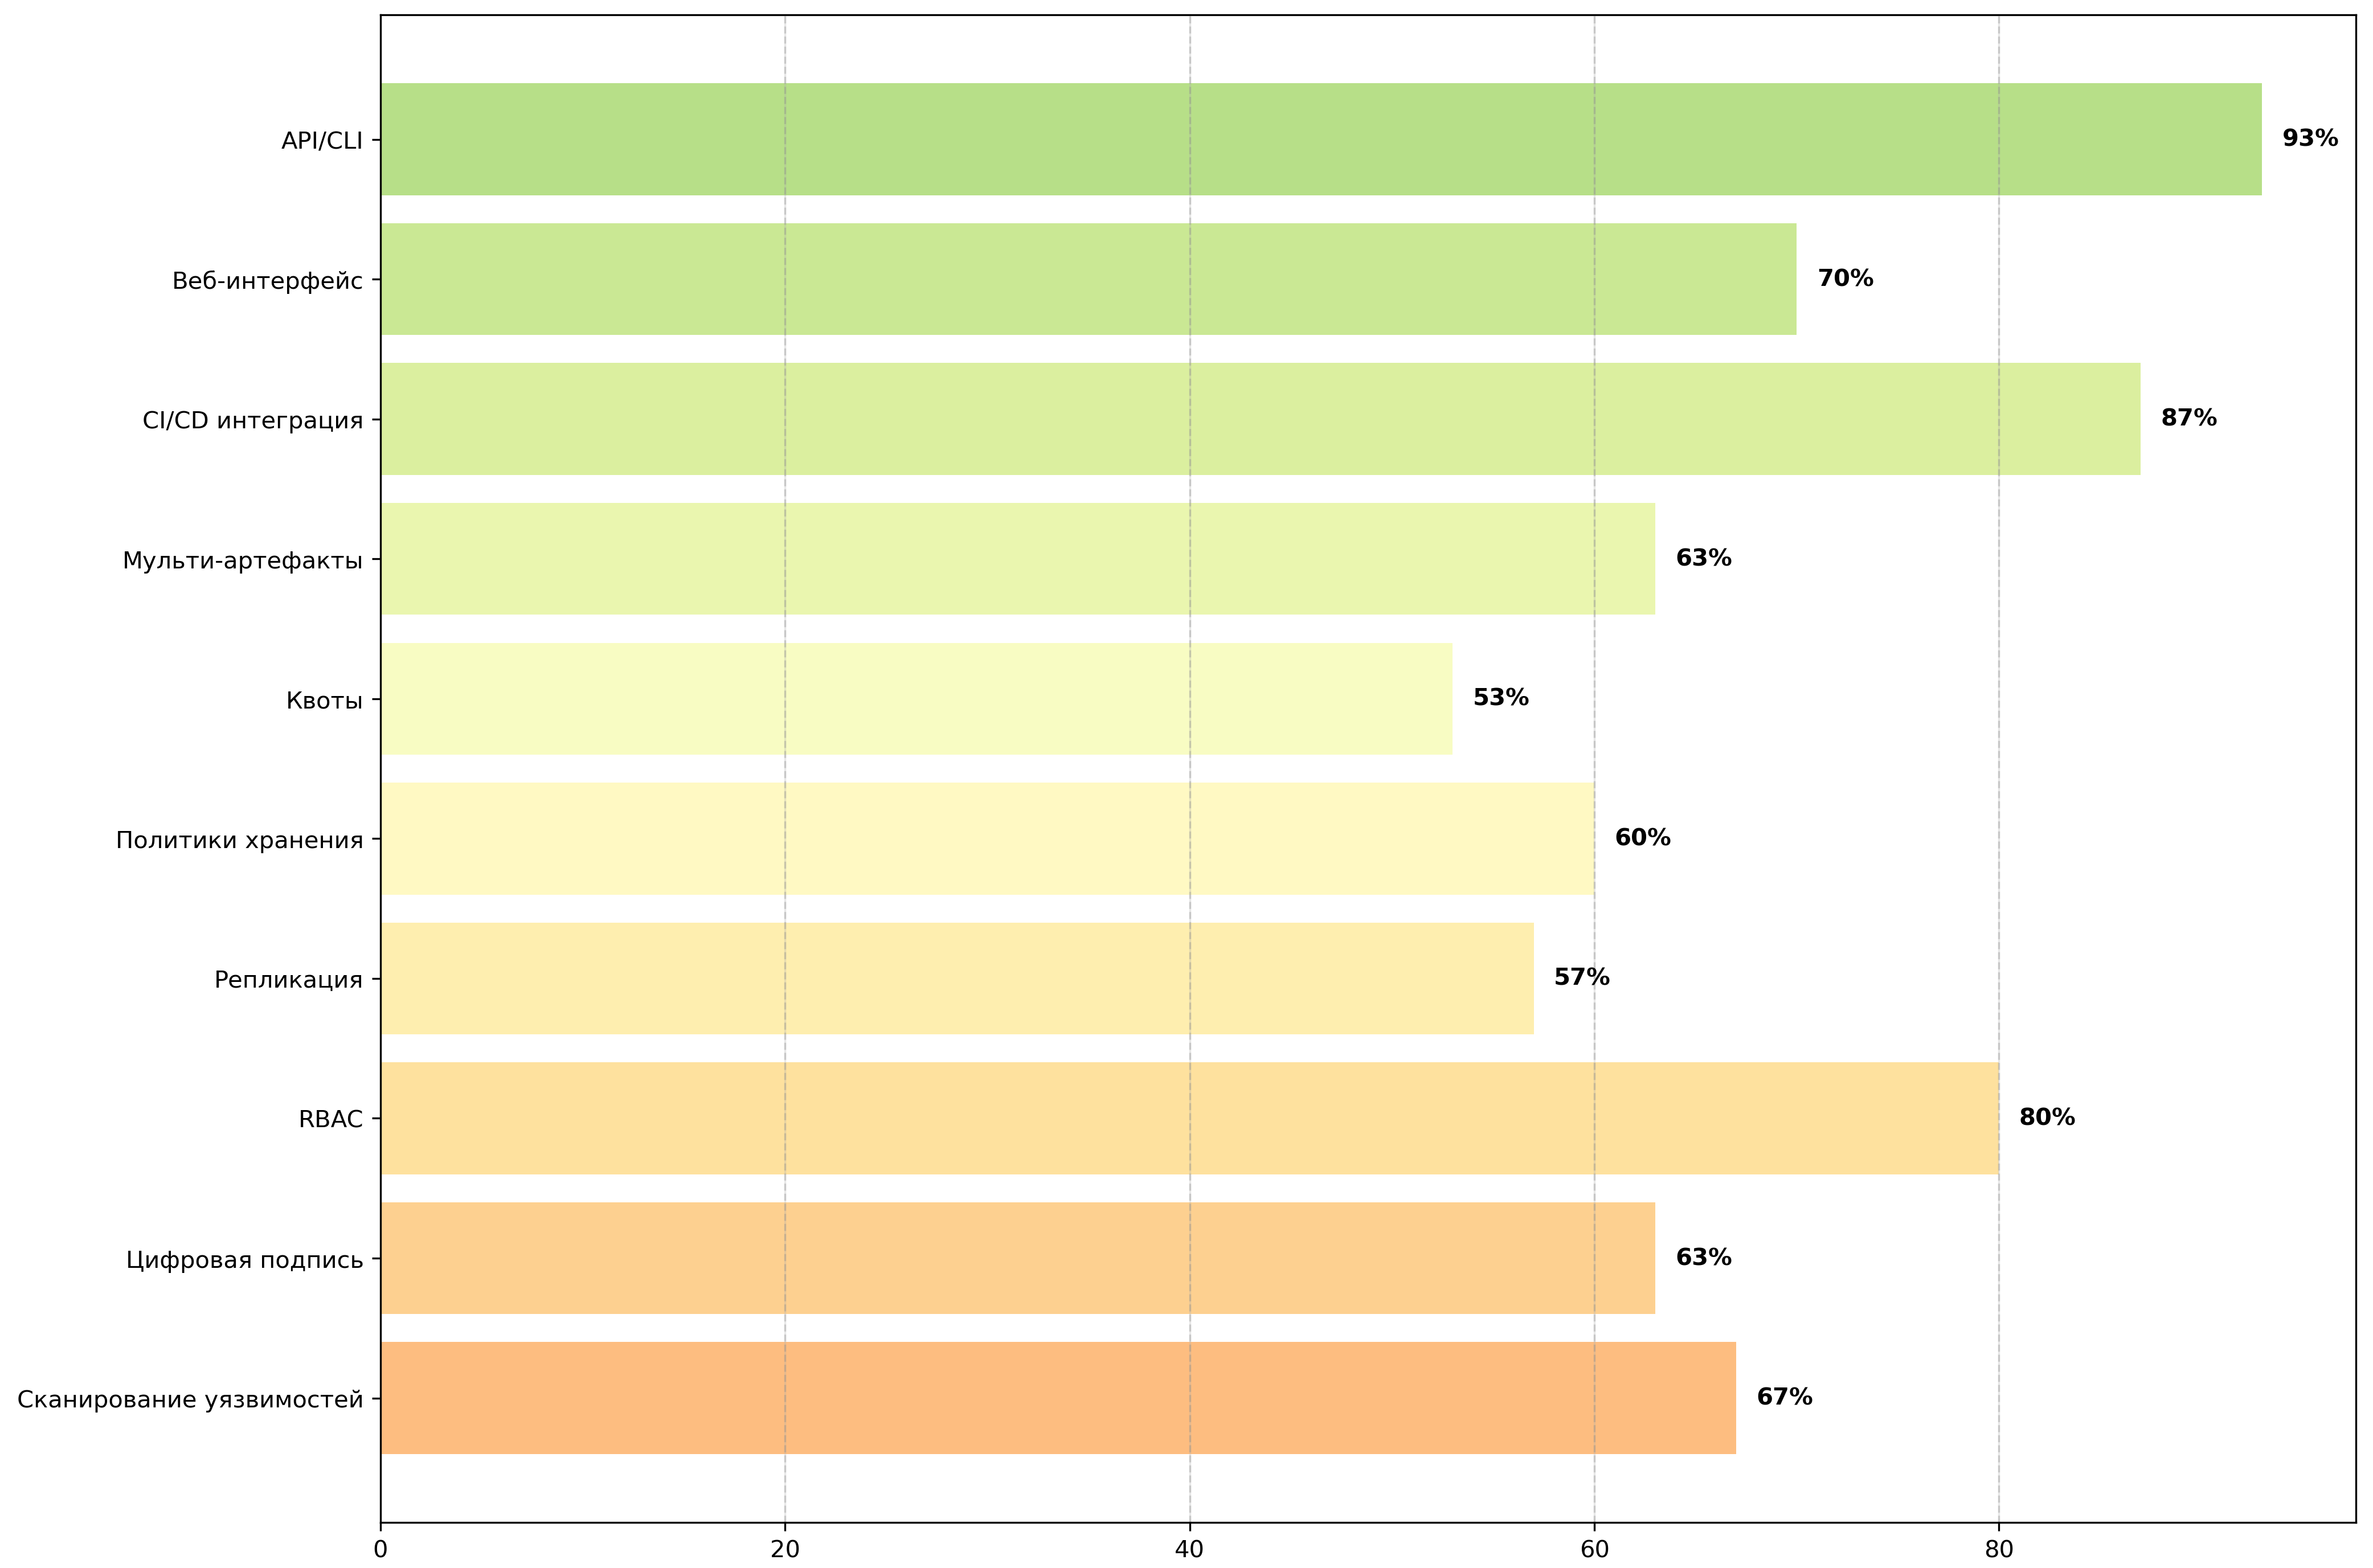
\includegraphics[width=0.9\textwidth]{analysis}
	\caption{Процент поддержки ключевых функций среди 30 систем управления реестрами}
	\label{fig:support-analysis}
\end{figure}

На основе проведенного анализа можно сформулировать следующие рекомендации:
\begin{enumerate}
	\item для организаций, ищущих открытое решение с полным функционалом, оптимальным выбором является Harbor;
	\item при использовании конкретного облачного провайдера целесообразно рассматривать его нативные сервисы (ECR, ACR, GCR);
	\item для крупных предприятий с комплексными требованиями подходят коммерческие решения JFrog Artifactory, Red Hat Quay Enterprise;
	\item Базовые решения Docker Registry пригодны только для тестовых сред и разработки
\end{enumerate}

Проведенное исследование подтвердило, что система Harbor является эталонным решением в категории open-source систем управления реестрами и может служить ориентиром при оценке других решений. Ее функциональность полностью покрывает требования корпоративной среды, что делает ее оптимальным выбором для организаций, seeking баланс между функциональностью, гибкостью и стоимостью владения.

\section{Интеграция Harbor в учебный процесс кафедры}
\label{subsec:harbor-education}

Система Harbor может быть интегрирована в учебный процесс для автоматизации проверки лабораторных работ и студенческих проектов. Практика создания тестовых пайплайнов уже давно применяется, однако интеграция системы Harbor позволит оптимизировать данный процесс.

Архитектура интеграции Harbor в учебный процесс включает несколько компонентов. Git-репозиторий содержит задания лабораторных работ, Dockerfile для сборки и тесты. Система Harbor выполняет роль приватного реестра для хранения базовых образов, образов с решениями студентов и тестовых образов. CI/CD система автоматизирует процессы сборки, тестирования и развертывания. Система мониторинга собирает результаты тестирования и метрики выполнения.

\subsection{Сценарий использования для лабораторных работ}

Процесс выполнения лабораторной работы начинается с того, что студент получает доступ к Git-репозиторию с заданием. Репозиторий содержит описание лабораторной работы, Dockerfile для сборки образа приложения, тесты для проверки корректности решения и конфигурационные файлы для CI/CD.

Студент разрабатывает решение и размещает его в личной ветке Git-репозитория. При отправке изменений запускается CI/CD пайплайн. Пайплайн собирает Docker-образ из решения студента, загружает образ Harbor в личный репозиторий студента, после чего запускает тестовый контейнер. Тестовый контейнер скачивает образ решения из Harbor, выполняет тесты в изолированном окружении и генерирует отчет о выполнении. Результаты тестирования публикуются в системе мониторинга.

Преподаватель получает доступ к результатам через веб-интерфейс Harbor.

\clearpage

\subsection{Пример реализации CI/CD пайплайна}

Для интеграции Harbor с GitLab CI может использоваться конфигурационный файл .gitlab-ci.yml. В листинге~\ref{lst:gitlab-ci} представлен пример конфигурации.

\begin{lstlisting}[caption={Пример .gitlab-ci.yml для лабораторной работы}, label={lst:gitlab-ci}, language=yaml, basicstyle=\small\ttfamily, frame=single, captionpos=b]
	stages:
	- build
	- test
	- deploy
	
	variables:
	HARBOR_URL: "harbor.bmstu.cloud"
	PROJECT: "iu7-labs"
	IMAGE_NAME: "lab1-app"
	
	build:
	stage: build
	image: docker:latest
	services:
	- docker:dind
	script:
	- docker build -t ${HARBOR_URL}/${PROJECT}/${IMAGE_NAME}:${CI_COMMIT_SHA} .
	- docker login -u ${HARBOR_USER} -p ${HARBOR_PASSWORD} ${HARBOR_URL}
	- docker push ${HARBOR_URL}/${PROJECT}/${IMAGE_NAME}:${CI_COMMIT_SHA}
	only:
	- branches
	
	test:
	stage: test
	image: docker:latest
	services:
	- docker:dind
	script:
	- docker login -u ${HARBOR_USER} -p ${HARBOR_PASSWORD} ${HARBOR_URL}
	- docker pull ${HARBOR_URL}/${PROJECT}/${IMAGE_NAME}:${CI_COMMIT_SHA}
	- docker run --rm ${HARBOR_URL}/${PROJECT}/${IMAGE_NAME}:${CI_COMMIT_SHA} python -m pytest tests/
	artifacts:
	reports:
	junit: test-results.xml
\end{lstlisting}

В этом примере определены три стадии: сборка, тестирование и развертывание. На стадии сборки создается Docker-образ из исходного кода студента, который затем загружается в Harbor. На стадии тестирования образ скачивается из Harbor и запускаются тесты с использованием pytest. Результаты тестирования сохраняются в формате JUnit для последующего анализа.

\clearpage
